\documentclass[11pt,a4paper]{scrartcl}
\usepackage[ngerman]{babel}
\usepackage[utf8]{inputenc}
\usepackage[T1]{fontenc}
\usepackage{graphicx}
\usepackage{float}
\usepackage{fullpage}
\usepackage{amssymb}
\usepackage{amsmath}
\usepackage[nounderscore]{syntax}
\usepackage{url}                % URLs
\usepackage{tikz}               % for the grey border on the title page
\usepackage{ziffer}				% to use commas as decimal separators in math mode
\usepackage{pdflscape}
\usepackage{multirow}
\usepackage{booktabs}
\usepackage{longtable, mdwtab}
\usepackage[absolute,overlay]{textpos}

\usepackage[a4paper,left=40mm,right=30mm,top=20mm,bottom=20mm,includeheadfoot]{geometry}
\newcommand{\changefont}[3]{\fontfamily{#1} \fontseries{#2} \fontshape{#3} \selectfont}
%\parindent 0pt
%\setlength{\parskip}{12pt}
\usepackage[raiselinks=true,
						bookmarks=true,
						bookmarksopenlevel=1,
						bookmarksopen=true,
						bookmarksnumbered=true,
						hyperindex=true,
						plainpages=false,
						pdfpagelabels=true,
						pdfborder={0 0 0.5},
						colorlinks=false,
						linkbordercolor={0 0.61 0.50},
						citebordercolor={0 0.61 0.50}]{hyperref}  %{0.57 0.74 0.57}

\author{PSE-Projekt 4 Team 2}
\title{Validierungsbericht zu Worthwhile}

\setcounter{tocdepth}{1} % make TOC fit on one page

\hyphenation{Worth-while}
\hyphenation{Pro-gramm-in-halt}

\newcommand{\reqtype}{}
\newenvironment{reqlist}[1]{\begin{description} \renewcommand{\reqtype}{#1}}{\end{description}}
\newcommand{\req}[3]{\item[\textbf{/\reqtype{}#1/}] #2 \\ #3}
\newcommand{\see}[1]{#1}
\renewcommand{\int}{\texttt{Integer}}
\newcommand{\bool}{\texttt{Boolean}}

\newcommand{\method}[1]{
			\item[\texttt{\textbf{#1}}]
            }
\newcommand{\attr}[1]{\item[\texttt{\textbf{#1}}]}
\newcommand{\type}[1]{\texttt{#1}}
\newcommand{\literal}[1]{\item[\texttt{#1}]}
\newcommand{\mlmethod}[1]{\method{\parbox{\textwidth}{#1}}}
\newenvironment{rcases}{%
  \left.\renewcommand*\lbrace.%
  \begin{cases}}%
{\end{cases}\right\rbrace}
\newcommand{\guitest}[5]{\subsubsection{#1}\begin{description}
	\item[Beschreibung] #2
	\item[Erwartetes Ergebnis] #3
	\item[Tatsächliches Ergebnis] #4
	\item[Gefundene Fehler/Anmerkungen] #5
\end{description}}
\graphicspath{{images/}}

\begin{document}

%% titlepage.tex
%%

% coordinates for the bg shape on the titlepage
\newcommand{\diameter}{20}
\newcommand{\xone}{-30}
\newcommand{\xtwo}{150}
\newcommand{\yone}{15}
\newcommand{\ytwo}{-265}

\begin{titlepage}
% bg shape
\begin{tikzpicture}[overlay]
\draw[color=gray]
 		 (\xone mm, \yone mm)
  -- (\xtwo mm, \yone mm)
 arc (90:0:\diameter pt)
  -- (\xtwo mm + \diameter pt , \ytwo mm)
	-- (\xone mm + \diameter pt , \ytwo mm)
 arc (270:180:\diameter pt)
	-- (\xone mm, \yone mm);
\end{tikzpicture}

	\begin{textblock}{10}[0,0](1.7,1)
		
\includegraphics[width=.3\textwidth]{images/kit_logo_de_4c_positiv.pdf}
	\end{textblock}
	\changefont{phv}{m}{n}	% helvetica	
	\begin{center}
		\fontsize{45}{50}\selectfont
        \vfill
        \textsc{Worthwhile} \\
        \textsc{Pflichtenheft}
        \vfill
		\LARGE
		PSE WS 11/12
  \vfill
 \newpage
 
 \null
 \vfill
 
 Praxis der Softwareentwicklung -- WS 2011/2010 \\
  Automatisches Prüfen der Korrektheit von Programmen \\
  Projekt 4 -- Gruppe 2 \\
  \medskip
  \vspace{2cm}
  \Large
  \begin{tabular}{|l|l|}
    \hline
    Leon Handreke & 123456 \\
    \hline
    Chris Hiatt & 1610922 \\
    \hline
    Stefan Orf & 123456 \\
    \hline
    Joachim Priesner & 1579308 \\
    \hline
    Fabian Ruch & 123456 \\
    \hline
    Matthias Wagner & 1579342 \\
    \hline
  \end{tabular}
  \vspace{2cm} \\
  \today \\
	Revision 0
	\end{center}
	
  \vfill

\end{titlepage}


\tableofcontents
\clearpage

\section{Zeitlicher Ablauf}

Im Großen und Ganzen hat sich die Zeitplanung aus der Entwurfsphase bewährt. Die Aufteilung in Aufgabenbereiche wurde weitestgehend eingehalten. Während der Entwicklung hat es sich als vorteilhaft erwiesen, eng ineinandergreifende Komponenten parallel zu entwickeln, um den geschriebenen Code sofort testen zu können. Im aktualisierten Gantt-Diagramm erscheinen deshalb einige Einheiten deutlich größer. Tatsächlich hat sich aus der Parallelisierung kein höherer Zeitaufwand ergeben. Trotzdem haben sich einige kleinere Änderungen im Laufe der Implementierungsphase ergeben, welche im Folgenden genauer dargestellt werden.

\subsection{Build-System}
Die Inbetriebnahme des Build-Systems sowie des Continous-Integration-Servers hat sich aufgrund einiger Schwierigkeiten bei der Konfiguration um einige Tage in die Weihnachtsferien hinein verschoben.

\subsection{Stubs und Unit-Tests}
Ursprünglich war geplant, vor der eigentlichen Implementierung Unit-Tests zu erstellen und die Klassen mit Stubs auszurüsten, welche die Tests erfolgreich ablaufen lassen. Da das Parsen von Testprogrammen jedoch bereits früh möglich war, wurden stattdessen parallel zur Implementierung Unit-Tests mit an den Testfall angepassten Testprogrammen geschrieben.

\subsection{Parser}
Aufgrund der Entscheidung, keine eigene Schnittstellenklasse zum Parser zu implementieren (siehe \ref{aenderung_parser}), sondern die von ANTLR generierte Klasse direkt zu verwenden, entfiel diese Aufgabe.

\subsection{Beweiserschnittstelle}
Die Abhängigkeit zwischen den Aufgaben "`Z3-Anbindung"' und "`SMTLIB-Kompilierung"' wurde aufgelöst, da es sich als vorteilhaft für die Zeiteinteilung herausstellte, beide parallel zu der aufwendigeren Formelgenerierung zu entwickeln.

\subsection{Interpreter}
Der Entschluss, alle Debug-Logik in einer seperaten "`Debugger"'-Komponente zu implementieren (siehe \ref{aenderung_interpreter_breakpoints}), führte dazu, dass die Einheit "`Breakpoints"' vom Aufgabenbereich "`Interpreter"' in den Aufgabenbereich der GUI-Entwicklung verschoben wurde.

\begin{landscape}%
	\begin{figure}%
		\vspace{-2cm}
		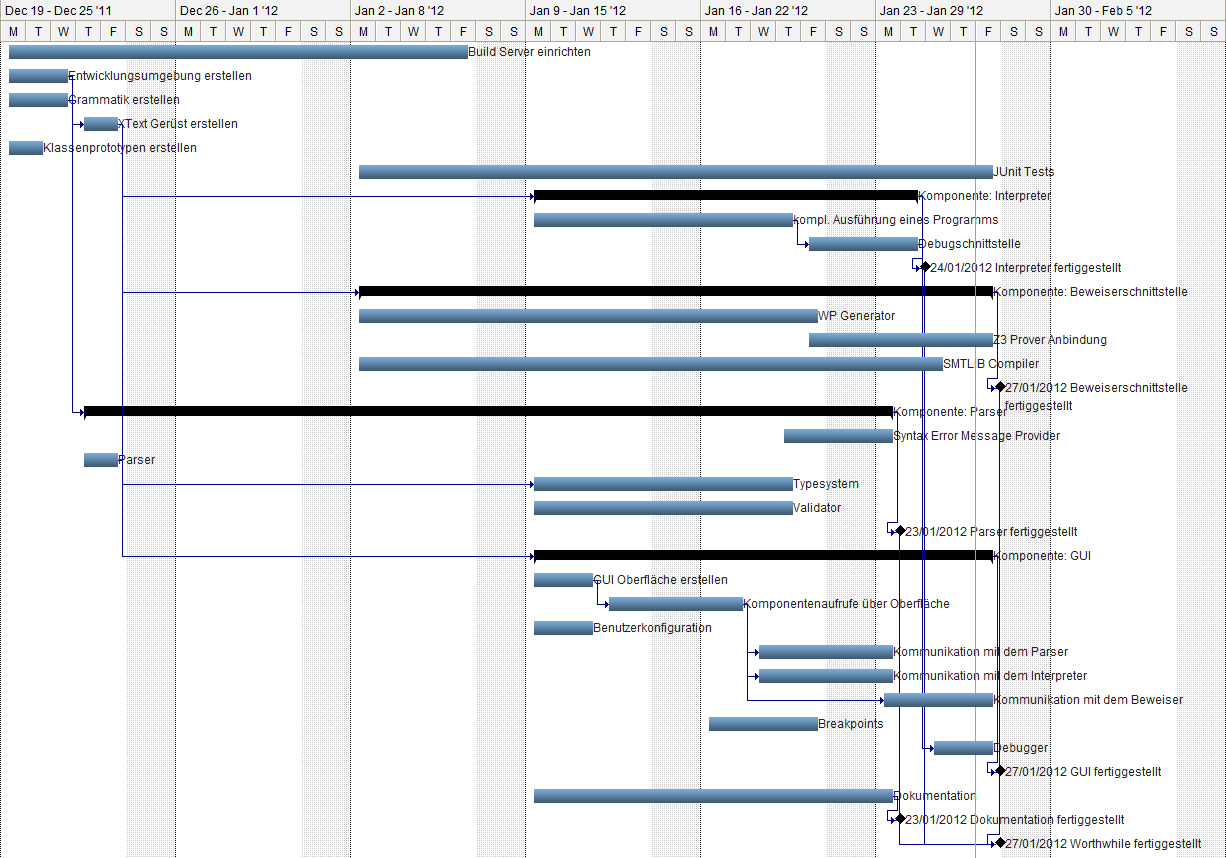
\includegraphics[height=1.2\textheight]{images/gantt_implementierung_diag.png}%
		\caption{Tatsächlicher Ablauf der Implementierungsphase.}%
	\end{figure}%
\end{landscape}

\section{Verwendete Werkzeuge}
\subsection{Bugtracker}
Um die Kommunikation innerhalb des Teams zu erleichtern und stets problembezogen zu gestalten, wurde bereits während der Implementierungsphase  die Bugtracking-Software "`GitHub Issues"' eingesetzt. Diese ist mit dem Quellcode-Repository integriert, sodass aus dem Bugtracker einfach auf Änderungen im Code verwiesen werden kann und sogar durch einen Eintrag in der Mitteilung zu einem Commit eine solche Referenz automatisch erzeugt werden kann.

Über den gesamten Entwicklungszeitraum hinweg wurden knapp über 100 Bugs angelegt. Davon bezogen sich etwa 30 auf die Benutzeroberfläche und jeweils ca. 20 auf die Beweiserschnittstelle und den Interpreter.

\subsection{Continous-Integration-Server}
Die Continous-Integration-Serversoftware Jenkins, die bereits während der Implementierungsphase verwendet wurde, um nach jeder Änderung die Kompilierbarkeit des Codes zu überprüfen, wurde auch in der Validierungsphase eingesetzt. Dabei wurden zusätzlich Plugins verwendet, die die Anzahl der Testfälle sowie die Anzahl der momentan erfolgreichen Tests grafisch anzeigen.

\begin{center}
	\begin{figure}[h] % place the figure here
		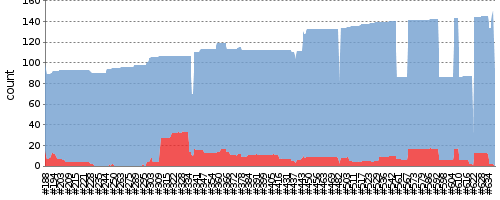
\includegraphics[width=13cm]{images/jenkins-test-trend.png}
		\caption{Entwicklung der Anzahl von Testfällen während der Validierungsphase}
	\end{figure}
\end{center}

\section{Überdeckungstests}
Zur Messung der Abdeckung des Codes durch die geschriebenen Testfälle wurde das Eclipse-Plugin EclEmma verwendet. Das Plugin hat gegenüber der Nutzung eines Programms auf der Kommandozeile den Vorteil, dass nicht durchlaufene Codezeilen in der Eclipse-Oberfläche markiert werden und so das Schreiben neuer Testfälle, die die Abdeckung erhöhen, vereinfacht wird.

Gemessen wurde die Abdeckung bei den Komponenten "`Beweiserschnittstelle"' und "`Interpreter"'. Diese Module enthalten einen Großteil der automatisch testbaren Logik in Worthwhile und sind komplett von den Komponenten "`Benutzeroberfläche"' und "`Debugger"' entkoppelt, die durch manuell ausgeführte Testszenarien getestet wurden. Es wurde sowohl Anweisungs- als auch Zweigüberdeckung gemessen.

Zusätzlich wurde auch die Überdeckung bei den manuellen GUI-Tests gemessen. Die zusammengefassten Überdeckungswerte der manuellen und der automatischen Testüberdeckung sind in Klammern angegeben.

\subsection{Beweiserschnittstelle}
In der Komponente "`Beweiserschnittstelle"' wurde eine Anweisungsüberdeckung von 75,4\% (78,1\%) und eine Zweigüberdeckung von 81,9\% (88,3\%) erreicht. Dabei wurde in \texttt{WPStrategy}, der Komponente, die den Weakest"=Precondition-Kalkül implementiert, sogar eine Zweigabdeckung von 93,8\% (100,0\%) erreicht. Durch die Verwendung des Visitor"=Entwurfsmusters wurden viele Fallunterscheidungen vermieden und damit das Testen in dieser Komponente stark vereinfacht.

\subsection{Interpreter}
In der Komponente "`Interpreter"' wurde eine Anweisungsüberdeckung von 78,8\% (88,5\%) und eine Zweigüberdeckung von 69,4\% (86,6\%) erreicht. Durch die vielfältige Auswahl von Testprogrammen wird dabei die Behandlung fast jedes Syntaxelementes mindestens einmal durchlaufen.

\subsection{Debugger}

Der Debugger wurde nur innerhalb der GUI-Tests getestet. Dort wurde eine Anweisungsüberdeckung von 86,8\% und eine Zweigüberdeckung von 76,8\% erreicht. Bedingt durch das Eclipse-Debugmodell werden viele allgemein gehaltene Interfaces implementiert, deren Funktionalität im Rahmen der Tests nicht voll ausgenutzt wird (beispielsweise das Abrufen des rohen Speicherinhalts im Debugger).

\subsection{GUI}

Bei den manuellen GUI-Tests erreichte die Komponente eine Anweisungsüberdeckung von 89,9\% und eine Zweigüberdeckung von 69,8\%. Die geringe Zweigüberdeckung resultiert vor allem aus dem Abfangen sehr seltener und schwer zu testender Fehlerbedingungen.
\section{Interationstests}

\section{GUI-Tests}

Ergebnisse der GUI-Tests siehe folgende Tabelle

\begin{landscape}

\begin{longtable}{lp{8cm}lp{10cm}}
\label{typesystemdef} \\
\caption{Resultate der GUI-Tests} \\
\toprule
\textbf{Testfall-Nr.} & \textbf{Beschreibung} & \textbf{Ergebnis} & \textbf{Gefundene Fehler/Anmerkungen} \\
\midrule
\midrule

\endhead

\endfoot

/T01/ & Randfälle korrekter Programme &  &  \\ \midrule
/T01a/ & Leeres Programm & OK & Beweiser meldet Erfolg zurück \\ \midrule
/T01b/ & Verschachteltes Programm & (OK) & \hyperlink{https://github.com/team-worthwhile/worthwhile/issues/30}{\hyperlink{https://github.com/team-worthwhile/worthwhile/issues/30}{Bug \#30}}: Stack overflow when validating very complex programs – behoben. Beweisen erst nach Heraufsetzen des Z3-Timeouts möglich \\ \midrule
/T01c/ & Langes Programm & (Fehlschlag) & Build des Programms dauert sehr lange, Abbruch \\ \midrule
/T01c/ (neu) & Langes Programm & OK & mit 5000 statt 10000 Zeilen \\ \midrule
\midrule
/T02/ & Fehlerhafte Programme &  &  \\ \midrule
/T02a/ & Falsch geschriebene/nicht existente Schlüsselwörter & OK &  \\ \midrule
/T02b/ & Fehlender Leerraum & OK &  \\ \midrule
/T02c/ & Fehlende/überflüssige Operanden & (OK) & \hyperlink{https://github.com/team-worthwhile/worthwhile/issues/54}{Bug \#54}: No red squiggly marker on syntax error at the end of statement \\ \midrule
/T02d/ & Operanden vom falschen Typ & (OK) & \hyperlink{https://github.com/team-worthwhile/worthwhile/issues/55}{Bug \#55}: Double error message in typesystem checker – behoben \\ \midrule
/T02e/ & Ungültige Parameter bei Funktionsaufruf & (OK) & \hyperlink{https://github.com/team-worthwhile/worthwhile/issues/56}{Bug \#56}: Empty array literal is assignable to scalar value – behoben \\ \midrule
/T02f/ & Aufrufen nicht deklarierter Funktionen & (OK) & \hyperlink{https://github.com/team-worthwhile/worthwhile/issues/75}{Bug \#75}: Validator tries to check parameter count on undeclared function \\ \midrule
/T02g/ & Verwenden nicht deklarierter Variablen & OK &  \\ \midrule
/T02h/ & Unerlaubte Typkonvertierung & OK &  \\ \midrule
\midrule
/T03/ & Syntaxhervorhebung & (OK) & \hyperlink{https://github.com/team-worthwhile/worthwhile/issues/31}{Bug \#31}: Inconsistent syntax highlighting of operators – behoben \\ \midrule
\midrule
/T04/ & Debuggen eines Programms &  &  \\ \midrule
/T04a/ &  - mit Abbruch des Programmablaufs & (OK) & \hyperlink{https://github.com/team-worthwhile/worthwhile/issues/76}{Bug \#76}: Stepping over loop or function call causes debugger to step over rest of program \\ \midrule
/T04b/ &  - mit Fortsetzen des Programmablaufs & (OK) & \hyperlink{https://github.com/team-worthwhile/worthwhile/issues/77}{Bug \#77}: Programs are not marked as terminated when reaching end of code \\ \midrule
/T04c/ &  - im Ausführungsmodus & OK &  \\ \midrule
\midrule
/T05/ & Ansprechbarkeit der Benutzeroberfläche & OK &  \\ \midrule
\midrule
/T06/ & Ändern von Variablenwerten während der Ausführung des Programms & (OK) & \hyperlink{https://github.com/team-worthwhile/worthwhile/issues/79}{Bug \#79}: WorthwhileExpressions.xmi not found when evaluating expressions \\ \midrule
\midrule
/T07/ & Korrekte Speicherung der Optionen &  &  \\ \midrule
\midrule
/T08/ & Testen des Überprüfens & & \hyperlink{https://github.com/team-worthwhile/worthwhile/issues/78}{Bug \#78}: Programs are not marked as terminated after proving \\ \midrule
/T08a/ & Testprogramm für Annotationen & OK &  \\ \midrule
/T08b/ & Programm mit verschachtelten Schleifen & OK &  \\ \midrule
/T08c/ & Rekursives Programm & -- & nicht anwendbar, da Sprache keine Rekursion erlaubt \\ \midrule
/T08d/ & Funktionsaufrufe in Annotationen & OK &  \\

\bottomrule
\bottomrule
\end{longtable}

\end{landscape}
\section{Profiling- und Performance-Tests}

Um einen Überblick über den Zeitaufwand der einzelnen Worthwhile-Komponenten zu gewinnen sowie zeitliche Hotspots zu identifizieren, wurden Profiling-Tests mit Unterstützung von VisualVM durchgeführt. Hierbei wurden einzelne, meist komplexere, Testprogramme aus der GUI gestartet und untersucht, um einen Eindruck von Worthwhile unter möglichst realen Bedingungen zu erlangen.

\subsection{Parser}

Das Parsen eines Programms ist abhängig von der Anzahl der vorkommenden Sprachkonstrukte. Beispielsweiße dauerte das Parsen des Programms bubblesort2.ww 111 ms. Eine eindeutige Aussage über die Dauer eines Parsevorgangs lässt sich schwer treffen, da die Anzahl sowie die Verschachtelungstiefe der Sprachkonstrukte eine große Rolle spielt. Jedoch benötigen die einzelne Sprachkonstrukte eine Bearbeitungszeit von Bruchteilen von Millisekunden bis hin zu wenigen Millisekunden. Im Testprogramm bubblesort2.ww stellte sich die Funktionsdeklaration mit 5,56 ms als am zeitaufwendigsten heraus.

\subsection{Interpreter}

Der Zeitbedarf für das Interpretieren ist genauso wie das Parsen abhängig von der Anzahl der Sprachkonstrukte. Jedoch muss hier nicht die Anzahl der vorkommenden sondern die der auszuführenden Elemente berücksichtigt werden. Deshalb lässt sich auch hier nicht eindeutig sagen wie viel Zeit ein Programm in der Ausführung benötigt, da insbesondere ein Prorgamm unter Umständen nie terminiert. Das Sortieren eines Arrays mit zehn Elementen mittels bubblesort2.ww benötigte etwa 18 Sekunden. Diese relativ hohe Zeit ist auf die ständig auftretenden Beweiseraufrufe zurück zu führen, welche annähernd 100 \% der Zeit ausmachten. Das Sortieren ohne die Beweiseraufrufe dauerte ca. 26 ms.

\subsection{Prover}

Das Überprüfen eines Testprogramms dauerte im Schnitt etwa 2 Sekunden. Am Beispiel der Testprogramme \texttt{test\_fibonacci.ww} und \texttt{bubblesort2.ww} lag die Beweiszeit bei 1865 ms bzw. 1895 ms. Da vor dem Beweisen ein Parsen des Codes und Typsystemüberprüfungen nötig sind, fallen etwa 100 bis 200 ms auf diese Aufgaben zurück. Die Transformation des Codes im wp-Kalkül benötigte für \texttt{bubblesort2.ww} 142 ms und für \texttt{test\_fibonacci.ww} 36 ms. Das Umwandeln einer einzelnen Annotation ins SMTLIB-Format betrug bei beiden Tests wenige Millisekunden (im Schnitt etwa 4 ms). Da jedoch die Annotationen einzeln umgewandelt und überprüft werden, liegt die Gesamtzeit der Umwandlungen ins SMTLIB-Format deutlich höher. Das Testprogramm \texttt{bubblesort2.ww} enthielt 13 und \texttt{test\_fibonacci.ww} 11 zu überprüfende Annotationen. Somit liegt der Zeitbedarf für das Umwandeln aller Annotation bei etwa 50 ms. Ebenso wird jede Annotation anschließend mittels externem Beweiser überprüft. Einzelne Annotationen zu beweisen, dauerte etwa 15 bis 17 ms und demnach lag der Gesamtzeitaufwand des Beweisers für das gesamte Programm bei 220 ms für \texttt{bubblesort2.ww} und bei 170 ms für \texttt{test\_fibonacci.ww}. Nach Überprüfung weiterer Testprogramme ergibt sich somit ein ungefährer Überblick über den anteiligen Zeitaufwand der Prover-Komponenten in Tabelle~\ref{zeitaufwandprover}.

\begin{table}[h]
\centering
\caption{Ungefährer Zeitaufwand der Prover-Komponenten}
\label{zeitaufwandprover}
\begin{tabular}{|l|l|}
\hline
\textbf{Komponente} & \textbf{Zeitaufwand} \\
\hline
Parser und Typsystem & 10\% \\
\hline
wp-Kalkül & 8\% \\
\hline
SMTLIB-Formatierung & 4\% \\
\hline
Beweiser (Z3) & 15\% \\
\hline
\end{tabular}
\end{table}

\section{Kompatibilitätstests}
Im Laufe der Entwicklung wurde Worthwhile auf die Kompatibilität mit verschiedenen Betriebssystemen, Rechnerarchitekturen und Java-Versionen getestet. Dabei wurde die Lauffähigkeit auf den Linux-Distributionen openSuse, Debian squeeze, Arch Linux, Fedora 14 sowie 16 und Gentoo sowie auf Windows 7 bestätigt. Bei einigen Tests wurde die offizielle Java-Implementation von Oracle verwendet, bei anderen die freie, auf OpenJDK basierende JVM "`IcedTea"' in Version 6 und 7. Mit keiner der verwendeten virtuellen Maschinen wurden Probleme festgestellt.

Wider Erwarten war es nötig, für Systeme mit Windows und Linux sowie für amd64- und i386-Architekturen die Software mit unterschiedlichen Parametern zu bauen. Dies ist auf verschiedene plattformspezifische Komponenten in der Eclipse-Plattform zurückzuführen, die beispielsweise je nach Plattform unterschiedliche Bibliotheken zum Zeichnen der Benutzeroberfläche verwendet. Der gesamte Worthwhile-spezifische Code hat sich als plattformunabhängig erwiesen.


\clearpage
\appendix

\end{document}
